\documentclass{beamer}
\usetheme{Boadilla}

\usepackage{tikz}
\usepackage{proof}
\usepackage{amsmath, amsthm, amssymb}

\newtheorem{thm}{Theorem}
\newtheorem{lem}{Lemma}
\newtheorem{cor}{Corollary}
\newtheorem{defn}{Definition}

\newcommand{\2}{\textbf{2}}
\newcommand{\A}{\mathcal{A}}
\newcommand{\G}{\mathcal{G}}
\newcommand{\Z}{\mathbb{Z}}
\newcommand{\N}{\mathbb{N}}
\newcommand{\Q}{\mathbb{Q}}
\newcommand{\p}{\mathfrak{A}}

\title{Abelian Automata and their Groups}
\author{Chris Grossack}
\date{July 20, 2018}

\begin{document}

\begin{frame}
\titlepage%
\end{frame}

\begin{frame}
  \tableofcontents%
\end{frame}

\section{Introduction}

\begin{frame}{Finite State Automata}
  \begin{itemize}
    \item Combinatorial Objects
    \item Encode functions as graphs
      \begin{itemize}
        \item states
        \item transitions
      \end{itemize}
  \end{itemize}

  \bigskip

  \begin{center}
  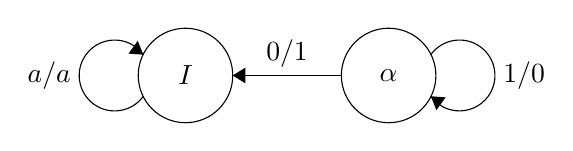
\begin{tikzpicture}[scale=0.2]
  \tikzstyle{every node}+=[inner sep=0pt]
  \draw [black] (23.2,-25.8) circle (3);
  \draw (23.2,-25.8) node {$I$};
  \draw [black] (36.1,-25.8) circle (3);
  \draw (36.1,-25.8) node {$\alpha$};
  \draw [black] (20.52,-27.123) arc (324:36:2.25);
  \draw (15.95,-25.8) node [left] {$a/a$};
  \fill [black] (20.52,-24.48) -- (20.17,-23.6) -- (19.58,-24.41);
  \draw [black] (33.1,-25.8) -- (26.2,-25.8);
  \fill [black] (26.2,-25.8) -- (27,-26.3) -- (27,-25.3);
  \draw (29.65,-25.3) node [above] {$0/1$};
  \draw [black] (38.78,-24.477) arc (144:-144:2.25);
  \draw (43.35,-25.8) node [right] {$1/0$};
  \fill [black] (38.78,-27.12) -- (39.13,-28) -- (39.72,-27.19);
  \end{tikzpicture}
  \end{center}

  \bigskip

  \begin{itemize}
    \item $\forall w \in \2^*~.~I(w) = w$\\
    \item $\forall w \in \2^\omega~.~I(w) = w$
    \item $\forall w \in \2^*~.~\alpha(w) = w+1$
  \end{itemize}
\end{frame}

\begin{frame}{Groups}
  \begin{itemize}
    \item Where we have functions, we have groups
    \item Interesting to automata theorists
      \begin{itemize}
        \item Study automata groups for their own structure 
      \end{itemize}
    \item Interesting to group theorists
      \begin{itemize}
        \item Rich source of counterexamples
        \item Compact way of encoding extremely complex groups
      \end{itemize}
  \end{itemize}

  \begin{defn}
    If $\A$ is an automaton with states $\{s_i\}$, then
    $\G(\A)$ is $\langle s_i \rangle$ 
  \end{defn}  
\end{frame}

\begin{frame}
  \begin{center}
  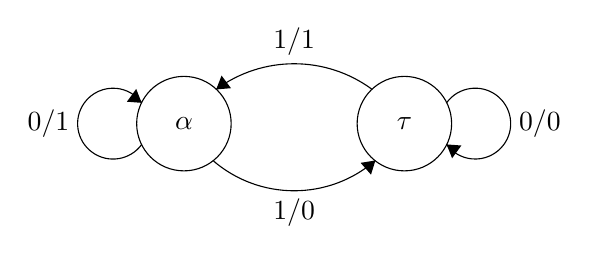
\begin{tikzpicture}[scale=0.2]
  \tikzstyle{every node}+=[inner sep=0pt]
  \draw [black] (22,-22.8) circle (3);
  \draw (22,-22.8) node {$\alpha$};
  \draw [black] (36,-22.8) circle (3);
  \draw (36,-22.8) node {$\tau$};
  \draw [black] (19.32,-24.123) arc (-36:-324:2.25);
  \draw (14.75,-22.8) node [left] {$0/1$};
  \fill [black] (19.32,-21.48) -- (18.97,-20.6) -- (18.38,-21.41);
  \draw [black] (34.155,-25.143) arc (-49.1226:-130.8774:7.878);
  \fill [black] (34.16,-25.14) -- (33.22,-25.29) -- (33.88,-26.04);
  \draw (29,-27.56) node [below] {$1/0$};
  \draw [black] (38.68,-21.477) arc (144:-144:2.25);
  \draw (43.25,-22.8) node [right] {$0/0$};
  \fill [black] (38.68,-24.12) -- (39.03,-25) -- (39.62,-24.19);
  \draw [black] (24.046,-20.628) arc (126.42271:53.57729:8.345);
  \fill [black] (24.05,-20.63) -- (24.99,-20.55) -- (24.39,-19.75);
  \draw (29,-18.5) node [above] {$1/1$};
  \end{tikzpicture}
  \end{center}

  \begin{itemize}
    \item This automaton generates the \textbf{Lamplighter Group} $\Z_2 \wr \Z$
    \item Finitely generated, not finitely presented
  \end{itemize}
\end{frame}

\begin{frame}
  
  \begin{center}
  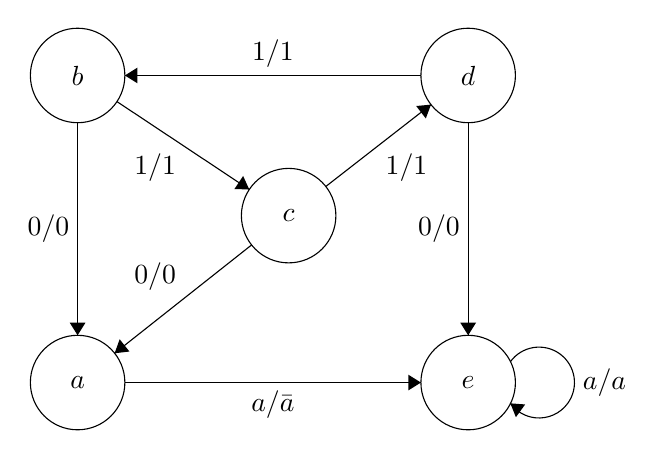
\begin{tikzpicture}[scale=0.2]
  \tikzstyle{every node}+=[inner sep=0pt]
  \draw [black] (14.4,-16.8) circle (3);
  \draw (14.4,-16.8) node {$b$};
  \draw [black] (14.4,-36.3) circle (3);
  \draw (14.4,-36.3) node {$a$};
  \draw [black] (39.2,-16.8) circle (3);
  \draw (39.2,-16.8) node {$d$};
  \draw [black] (39.2,-36.3) circle (3);
  \draw (39.2,-36.3) node {$e$};
  \draw [black] (27.8,-25.7) circle (3);
  \draw (27.8,-25.7) node {$c$};
  \draw [black] (17.4,-36.3) -- (36.2,-36.3);
  \fill [black] (36.2,-36.3) -- (35.4,-35.8) -- (35.4,-36.8);
  \draw (26.8,-36.8) node [below] {$a/\bar{a}$};
  \draw [black] (41.88,-34.977) arc (144:-144:2.25);
  \draw (46.45,-36.3) node [right] {$a/a$};
  \fill [black] (41.88,-37.62) -- (42.23,-38.5) -- (42.82,-37.69);
  \draw [black] (39.2,-19.8) -- (39.2,-33.3);
  \fill [black] (39.2,-33.3) -- (39.7,-32.5) -- (38.7,-32.5);
  \draw (38.7,-26.55) node [left] {$0/0$};
  \draw [black] (36.2,-16.8) -- (17.4,-16.8);
  \fill [black] (17.4,-16.8) -- (18.2,-17.3) -- (18.2,-16.3);
  \draw (26.8,-16.3) node [above] {$1/1$};
  \draw [black] (14.4,-19.8) -- (14.4,-33.3);
  \fill [black] (14.4,-33.3) -- (14.9,-32.5) -- (13.9,-32.5);
  \draw (13.9,-26.55) node [left] {$0/0$};
  \draw [black] (16.9,-18.46) -- (25.3,-24.04);
  \fill [black] (25.3,-24.04) -- (24.91,-23.18) -- (24.36,-24.01);
  \draw (19.32,-21.75) node [below] {$1/1$};
  \draw [black] (25.45,-27.56) -- (16.75,-34.44);
  \fill [black] (16.75,-34.44) -- (17.69,-34.33) -- (17.07,-33.55);
  \draw (19.32,-30.5) node [above] {$0/0$};
  \draw [black] (30.16,-23.85) -- (36.84,-18.65);
  \fill [black] (36.84,-18.65) -- (35.9,-18.74) -- (36.51,-19.53);
  \draw (35.28,-21.75) node [below] {$1/1$};
  \end{tikzpicture}
  \end{center}

  \begin{itemize}
    \item This automaton generates the \textbf{Grigorchuk Group}, 
          the first constructive example of a group of intermediate growth
  \end{itemize}
\end{frame}

\section{Abelian Automata}
\begin{frame}
  \begin{defn}
    For $f \in \A$, $f_0$ is the state after following a 0 transition.
    Similarly $f_1$ is the state after following a 1 transition.
    This extends naturally to functions $f \in \G(\A)$.
  \end{defn}

  \begin{defn}
    A function $f \in \G(\A)$ is called \textbf{odd} if it toggles
    the first bit it reads, and \textbf{even} otherwise.
  \end{defn}

  \begin{defn}
    An automaton $\A$ is called \textbf{Abelian} if the group it generates is
  \end{defn}

  \begin{thm}[Sutner]
    $\A$ is abelian iff $\exists \gamma$ such that 
    $\forall f \in \G(\A)$ 
    \[
      f_0^{-1}f_1 = 
      \begin{cases}
        I      & f \text{ is even}\\
        \gamma & f \text{ is odd}\\
      \end{cases}
    \]
  \end{thm}
\end{frame}

\begin{frame}
  \begin{thm}[Nekrashevich and Sidki (paraphrased)]
    Every abelian automaton group is isomorphic to either an 
    integer lattice or a boolean group. 
    Further, when isomorphic to an integer lattice, residuation
    lifts to a matrix operation.
  \end{thm}

  \begin{itemize}
    \item This means we can consider $\G(\A) \cong \Z^m$, 
      equipped with a matrix $A$ which encodes residuation in the 
      following way:
    \item $\partial_0:f \mapsto f_0$ lifts to an affine function:
      \[
        v_0 = 
        \begin{cases}
          A(v)   & v \text{ is even}\\
          A(v-r) & v \text{ is odd}\\
        \end{cases}
      \]
    \item $\partial_1:f \mapsto f_1$ is similar:
      \[
        v_1 = 
        \begin{cases}
          A(v)   & v \text{ is even}\\
          A(v+r) & v \text{ is odd}\\
        \end{cases}
      \]
    \item Somewhat annoyingly, $r$ can be any odd vector\ldots
      \begin{itemize}
        \item Infinitely many linear algebraic interpretations of one machine
      \end{itemize}
  \end{itemize}
\end{frame}

\begin{frame}
  \begin{thm}[N+S (paraphrased)]
    $\chi_A$ is Q-irreducible exactly when your automata use prime many digits
  \end{thm}

  \begin{lem}
    2 is prime
  \end{lem}

  \begin{cor}
    For the matrices of interest to us, $\chi_A$ is Q-irreducible.
  \end{cor}
\end{frame}

\section{Module Theoretic Background}
\begin{frame}{Module Theory}
  \begin{itemize}
    \item $\Z^m$ looks kind of like $\Q^m$
    \item $\Z^m$ comes equipped with a matrix $A$ of irreducible character\ldots
    \item This may remind you of viewing $\Q^m$ as a cyclic $\Q[x]$ module
  \end{itemize}

  \begin{defn}
    A \textbf{module} $M$ over a ring $R$ is a really bad vector space.
    Just like you can scale vectors by coefficients coming from some field, 
    we can scale module elements by coefficients coming from some ring.\\
    If $r_1, r_2 \in R$ and $x,y \in M$, then we require things be nice:
    \begin{itemize}
      \item $r_1 \cdot (x+y) = r_1 \cdot x + r_1 \cdot y$
      \item $(r_1 + r_2) \cdot x = r_1 \cdot x + r_2 \cdot x$
      \item $(r_1r_2) \cdot x = r_1 \cdot (r_2 \cdot x)$
    \end{itemize}
  \end{defn}
\end{frame}

\begin{frame}
  \begin{thm}
    If $\A$ is an abelian automaton, then $\G(\A) \cong \Z^m$ is a $\Z[x]$ 
    module, where $p \cdot v = p(A^{-1})v$
  \end{thm}

  \begin{thm}
    $\G(\A)$ is actually a \textbf{cyclic} $\Z[x]$ module, namely:
    \[
      \forall v \in \Z^m, \exists p \in \Z[x] \text{ such that } v = p \cdot e_1
    \]
  \end{thm}
\end{frame}

\begin{frame}
  \begin{itemize}
    \item Now we can characterize the different residuation vectors!
    \item Recall for any odd vector $r$:
      \begin{itemize}
        \item $\partial_0:f \mapsto f_0$ lifts to an affine function:
          \[
            v_0 = 
            \begin{cases}
              A(v)   & v \text{ is even}\\
              A(v-r) & v \text{ is odd}\\
            \end{cases}
          \]
      \end{itemize}
    \item But our group is a cyclic module, so instead of $A(v-r)$, 
          consider $A(v - p \cdot e_1)$
    \item Then if $v = p \cdot u$, 
          $A(p \cdot u - p \cdot e_1) = p \cdot A(u - e_1)$
    \item So really, different residuation vectors correspond to 
          various extensions of some initial group, $\p$
          generated when $r = e_1$.
  \end{itemize}
\end{frame}

\begin{frame}{extensions?}
  \begin{defn}
    Denote by $p \cdot \p$ the automaton group $\Z^m$ whose 
    residuation is given by
      \[
        v_0 = 
        \begin{cases}
          A(v)   & v \text{ is even}\\
          A(v-r) & v \text{ is odd}\\
        \end{cases}
      \]
    Note that since $r$ must be an odd vector, 
    $p$ must have odd constant term.
  \end{defn}

  \begin{thm}
    If $p | q$ then $p \cdot \p \leq q \cdot \p$. 
    In particular, $\forall p~.~\p \leq p \cdot \p$
  \end{thm}
\end{frame}

\begin{frame}
  \begin{proof}[Hand-Wavy Proof$^{\text{TM}}$]
    Let $f \in p \cdot \p$. It suffices to find $g \in q \cdot \p$
    such that $f$ and $g$ have the same parity and have equal
    residuals.

    \bigskip

    Let $q = mp$ by assumption. Then $g = m \cdot f$ works.

    \bigskip

    Since $q$ and $p$ have odd constant term, so must $m$\\
    ``odd times even is even, odd times odd is odd''\\
    Clearly, then, $g$ and $f$ have the same parity.

    \bigskip

    If $f$ is even, then $f_0 = Af$ and\\
    $g_0 = (m \cdot f)_0 = A(m \cdot f) = m \cdot (Af) = m \cdot f_0$

    \bigskip

    If $f$ is odd, then $f_0 = A(f - p \cdot e_1)$ and\\
    $g_0 = (m \cdot f)_0 = A(m \cdot f - q \cdot e_1) = m \cdot A(f - p \cdot e_1) = m \cdot f_0$

    \bigskip

    So, by induction we are done.
  \end{proof}
\end{frame}

\begin{frame}{What about other vectors?}
  \begin{itemize}
    \item $p \cdot v \in p \cdot \p$ is the same function as $v \in \p$
    \item What about vectors which can NOT be written as $p \cdot v$?
    \item They are \textbf{Fractional}. They correspond to 
          vectors $v \in \Q^m$ such that $p \cdot v \in \Z^m$. 
    \item This justifies the idea of an \emph{extension} of $\p$. 
          Every time we scale by a polynomial, we introduce new group
          elements, which are fractions of the original group elements.
  \end{itemize}
\end{frame}

\section{Using the theory}
\begin{frame}
  \begin{itemize}
    \item What we've seen so far is a cool characterization of these groups
    \item Can we solve problems with it, though?
  \end{itemize}

  \begin{defn}[Orbit Problem]
    Given a function $f$ from some abelian automaton group, and
    words $x, y \in \2^*$ (or polite words in $\2^\omega$), 
    does there exist a $t \in \Z$ such that $f^t(x) = y$?
  \end{defn}
\end{frame}

\begin{frame}
  \begin{itemize}
    \item We start with the finite case.
    \item Identify $f$ with a vector in $p \cdot \p$ for some
          principal group $\p$.
  \end{itemize}

  \begin{defn}
    For $u \in \2^*$ let $\langle u \rangle = v \in p \cdot \p$ such that
    $v(0^{|u|}) = u$
  \end{defn}
\end{frame}

\begin{frame}
  \begin{thm}
    $\langle u \rangle$ always exists, and is unique mod 
    $\textbf{Stab}(0^{|u|})$
  \end{thm}

  \begin{lem}
    Denote $p \cdot e_1 \in p \cdot \p$ by $\delta$, and 
    let $u0v$ be a word in $\2^*$ (or $\2^\omega$) with $|u| = n$.
    \[
      (x^{n} \cdot \delta)(u0v) = u1v
    \]
  \end{lem}

  \begin{proof}
    When $n = 0$, notice $\delta(0v)$ = $1v$ since $\delta$ is odd and
    $\delta_0 = A(\delta - p \cdot e_1) = 0$.

    \bigskip

    Otherwise, $x^{n+1} \cdot \delta = x \cdot x^{n} \cdot \delta$.\\
    One can check $(x^{n+1} \cdot \delta)$ is even and further
    $(x^{n+1} \cdot \delta)_0 = (x^{n} \cdot \delta)$
    
    \bigskip

    Then $(x \cdot x^{n} \cdot \delta)(u_0u0v) = u_0 (x^{n} \cdot \delta)(u0v) = u_0(u1v)$
  \end{proof}
\end{frame}

\begin{frame}
  \begin{proof}
    For $u \in \2^*$, $\langle u \rangle = (\sum_{i=0}^{|u|-1}u_i x^i) \cdot \delta$ works\\

    \medskip

    (Recall we want $\langle u \rangle (0^{|u|}) = u$)

    \bigskip

    By the lemma, each $x^i \cdot \delta$ flips the $ith 0$ to a $1$,
    and leaves everything else unchanged. Since each $u_i$ is a $1$ iff
    it needs to be flipped, the polynomial works.

    \bigskip

    Uniqueness mod $\textbf{Stab}(0^{|u|})$ follows from basic group theory.
  \end{proof}
\end{frame}

\begin{frame}
  \begin{thm}[Finite Orbit Problem]
    The orbits of $f$ corresopnd precisely to lines in $\Z^m$.
  \end{thm}

  \begin{proof}
    Let $u \in \2^*$. Then $\langle(tf)u\rangle = tf + \langle u \rangle$

    \bigskip

    Thus, the orbit of $u$ under $f$ is precisely 
    $(\Z f + \langle u \rangle)(0^{|u|})$
  \end{proof}
\end{frame}

\begin{frame}{What about when $u \in \2^\omega$?}
  \begin{itemize}
    \item The above proof breaks becase $\langle u \rangle$ is not well
          defined on $\2^\omega$
    \item However we can approximate $u \in \2^\omega$ as a sequence of 
          strings of increasing length.
    \item If we can create a sequence of functions which sends each $0$
          string to the appropriate $u$ approximation, then our sum will
          converge in the cantor topology, and we can run the same 
          orbit argument.
  \end{itemize}
\end{frame}

\begin{frame}
  \begin{thm}
    $\langle u \rangle = (\sum_i u_i x^i) \cdot \delta$ works.
  \end{thm}

  \begin{itemize}
    \item For cardinality reasons, however, this clearly 
          can't always converge in our group.
    \item $\2^\omega$ is uncountable, $p \cdot \p$ is clearly countable
          for all $p$.
  \end{itemize}
\end{frame}

\begin{frame}
  \begin{defn}
    $u \in \2^\omega$ is called \textbf{ultimately periodic} iff $u = tv^*$
    for some $|t|, |v| < \infty$
  \end{defn}

\begin{itemize}
  \item Does every ultimately periodic word $u$ have a well defined $\langle u \rangle$?
  \item Is every word $u$ with well defined $\langle u \rangle$ ultimately periodic?
\end{itemize}

  \begin{thm}
    Yes.
  \end{thm}
\end{frame}

\begin{frame}
  \begin{proof}
    let $u = tv^*$, then the polynomial we would associate to 
    $\langle u \rangle$ is 
    \begin{align*}
      \langle u \rangle &= (\sum_i u_i x^i) \cdot \delta\\
                        &= \left ( \sum_{i<|t|} t_i x^i + x^{|t|} \frac{\sum_{i<|v|} v_i x^i}{1 - x^{|v|}} \right ) \cdot \delta\\
                        &= \left ( \langle t \rangle + x^{|t|} \frac{\langle v \rangle}{1 - x^{|v|}} \right ) \cdot \delta\\
                        &= \frac{p_1}{p_2} \cdot \delta\\
                        &= p_1 \cdot \delta \in p_2 \cdot \p
    \end{align*}

    It is easy to see that any function applied to $0^\omega$ gives a ultimately periodic string,
    completing the proof.
  \end{proof}
\end{frame}
\end{document}
